\section{111 --- Minimum Depth of Binary Tree}
Given a binary tree, find its minimum depth.

The minimum depth is the number of nodes along the shortest path from the root node down to the nearest leaf node.

\textbf{Note}: A leaf is a node with no children.

\paragraph{Example:}
\begin{flushleft}

Given binary tree \fcj{[3,9,20,null,null,15,7]},

\begin{figure}[H]

\begin{figure}[H]
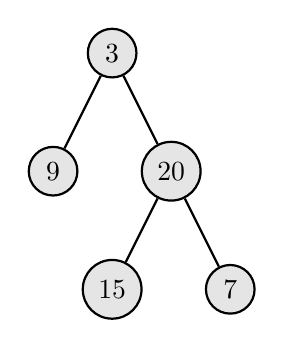
\begin{tikzpicture}
[every node/.style={draw, circle, fill=gray!20!, minimum size=5mm},
%level 1/.style={sibling distance=25mm},
%level 2/.style={sibling distance=15mm},
thick]
\node{3}
child{node{9}}
child{node{20} child{node{15}} child{node{7}}};
\end{tikzpicture}
\end{figure}

\end{figure}
return its minimum \fcj{depth = 2}.
\end{flushleft}

\subsection{Depth First Search}
We incorporate find balance into calculate depth. If we find each node has unbalanced left and right child tree, we return a negative number.

\setcounter{lstlisting}{0}
\begin{lstlisting}[style=customc, caption={DFS}]
bool isBalanced( TreeNode* root )
{
    auto res = depth( root );
    return res >= 0;
}
//helper function to find depth of a node
//we incorprate into comparing depth of left and right
//child tree
//when it is not balance,
//return -1
int depth( TreeNode* node )
{
    if( !node )
    {
        return 0;
    }
    int l_dep = depth( node->left );
    if( l_dep < 0 )
    {
        return -1;
    }

    int r_dep = depth( node->right );
    if( r_dep < 0 )
    {
        return -1;
    }
    //check if left and right child tree
    //are balanced
    int diff = abs( l_dep - r_dep );
    if( diff > 1 )
    {
        //unbalanced
        return -1;
    }
    //balanced
    //return the depth
    return ( max )( l_dep, r_dep ) + 1;
}
\end{lstlisting}
